\subsection{Binary Diffing}
\begin{frame}
    \frametitle{What is it?}
    \begin{itemize}
        \item The science of comparing similar binaries to pinpoint changes
            \pedbullet{Ex: Comparing the vulnerable and patched versions of a DLL}
        \item Byte level comparisons fail for a number of reasons
            \pedbullet{Compiler optimizations}
            \pedbullet{Branch inversion}
            \pedbullet{A single added line of source code or structure variable can change register usage, instruction ordering, offsets etc}
    \end{itemize}
\end{frame}

\begin{frame}
    \frametitle{Approaches to Bin Diffing}
    \begin{itemize}
        \item Binary and function heuristics
        \item Graph isomorphism
        \item Graph heuristics
            \pedbullet{Halvar Flake's work is most notable in this field, has turned into a commercial product and is described in more detail in the coming slides}
    \end{itemize}
\end{frame}

\begin{frame}
    \frametitle{Zynamics High Level Algorithm}
    \begin{itemize}
        \item Function level heuristics
            \pedbullet{Node, edge and call count}
            \pedbullet{Small primes product}
        \item Node level heuristics
            \pedbullet{Number of blocks in the shortest path to the entry / exit point, call count}
            \pedbullet{Small primes product}
        \item Instruction level heuristics
            \pedbullet{Distance to node entry / exit point}
        \item Small primes product
            \pedbullet{Create a table of small prime numbers}
            \pedbullet{Use the instruction opcode as an index into the table}
            \pedbullet{Keep a running product}
            \pedbullet{Wrap at long long}
    \end{itemize}
\end{frame}

\begin{frame}
    \frametitle{Application in Malware Analysis}
    \begin{itemize}
        \item Bin Diffing can be used to align functions between variants of malcode and port both names and comments
        \item Consider the situation where you have spent hours analyzing a binary
            \pedbullet{Analysis time can be saved by porting symbols}
            \pedbullet{Analysis time can be saved by pinpointing the exact changes}
        \item Fortunately for the malcode analysts, Bin Diffing malware samples tends to be easier than patch analysis
    \end{itemize}
\end{frame}

\subsection{Example in Malware Analysis}

\begin{frame}
    \frametitle{Invoking BinDiff}
    \begin{itemize}
        \item \emph{BinDiff} presents the following dialog when the plug-in is invoked in \emph{IDA}
      \begin{center}
        \pgfimage<1>[height=5cm]{images/binary_diffing/bindiff_01_start}
      \end{center}
    \end{itemize}
\end{frame}

\begin{frame}
    \frametitle{BinDiff Primary Signature Cache}
    \begin{itemize}
        \item \emph{BinDiff} will first generate signatures out of the current \emph{IDB} and the one selected to diff against
      \begin{center}
        \pgfimage<1>[height=3cm]{images/binary_diffing/bindiff_02_building_signature}
      \end{center}
    \end{itemize}
\end{frame}

\begin{frame}
    \frametitle{BinDiff Fixed Points}
    \begin{itemize}
        \item \emph{BinDiff} will then generate points from which to start matching and will go through several rounds of processing until the set of functions to match is exhausted
      \begin{center}
        \pgfimage<1>[height=3cm]{images/binary_diffing/bindiff_03_working}
      \end{center}
    \end{itemize}
\end{frame}


\begin{frame}
    \frametitle{BinDiff Results}
    \begin{itemize}
        \item Once \emph{BinDiff} has completed the matching, it will present three windows, one with the functions that couldn't be matched in the current \emph{IDB}, another with the unmatched functions in the second \emph{IDB} and finally a window showing the matched functions
      \begin{center}
        \pgfimage<1>[height=4.5cm]{images/binary_diffing/bindiff_04_results}
      \end{center}
    \end{itemize}
\end{frame}

\begin{frame}
    \frametitle{Close Inspection}
    \begin{itemize}
        \item It's also possible to investigate basic block and instruction level changes in order to try to discover the specific changes
      \begin{center}
        \pgfimage<1>[height=5cm]{images/binary_diffing/bindiff_05_graph_results}
      \end{center}
    \end{itemize}
\end{frame}

\begin{frame}
    \frametitle{Close Inspection}
    \begin{itemize}
        \item BinDiff 2 also offers a line by line assembly view of the changes
      \begin{center}
        \pgfimage<1>[height=5cm]{images/binary_diffing/bindiff_06_asm_results}
      \end{center}
    \end{itemize}
\end{frame}


\subsection{Binary Matching}
\begin{frame}
    \frametitle{Phylogenetic Classification}
    \begin{itemize}
        \item Binary comparison via graph similarities
            \pedbullet{Same heuristics as binary diffing}
        \item Application of clustering analysis to create taxonomy
        \item Define a similarity function that yields: 0 $<$= value $<$= 1
            \pedbullet{Near 0 indicates a low degree of resemblance}
            \pedbullet{Near 1 indicates a high degree of resemblance}
    \end{itemize}
    \begin{center}
        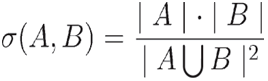
\includegraphics[scale=.33]{images/binary_diffing/similarity_function.png} \\
    \end{center}
    \begin{itemize}
        \item By maintaining large trees of malware, new and unidentified malware can  be immediately assigned into a family for classification and porting
    \end{itemize}
\end{frame}

\begin{frame}
    \frametitle{Phylogenetic Classification}
    \begin{itemize}
        \item Using the previously defined equation, distance matrices can be generated:
    \end{itemize}
    \begin{center}
    \begin{tiny}
    \begin{tabular}{l|rrrrrr}
                 & mimail.a & mimail.b & mimail.c & mimail.d & mimail.e & mimail.f \\ \hline
        mimail.a & 0        & 90.8     & 85.4     & 87.4     & 75.0     & 75.0     \\
        mimail.b & 90.8     & 0        & 84.7     & 88.0     & 74.3     & 74.3     \\
        mimail.c & 85.4     & 84.7     & 0        & 81.5     & 81.3     & 81.3     \\
        mimail.d & 87.4     & 88.0     & 81.5     & 0        & 72.3     & 72.3     \\
        mimail.e & 75.0     & 74.3     & 81.3     & 72.3     & 0        & 95.4     \\
        mimail.f & 75.0     & 74.3     & 81.3     & 72.3     & 95.4     & 0        \\
    \end{tabular}
    \end{tiny}
    \end{center}
\end{frame}

\begin{frame}
    \frametitle{Phylogenetic Classification}
    \begin{itemize}
        \item X-tree clustering algorithm can be applied to distance matrices
    \end{itemize}
    \begin{center}
        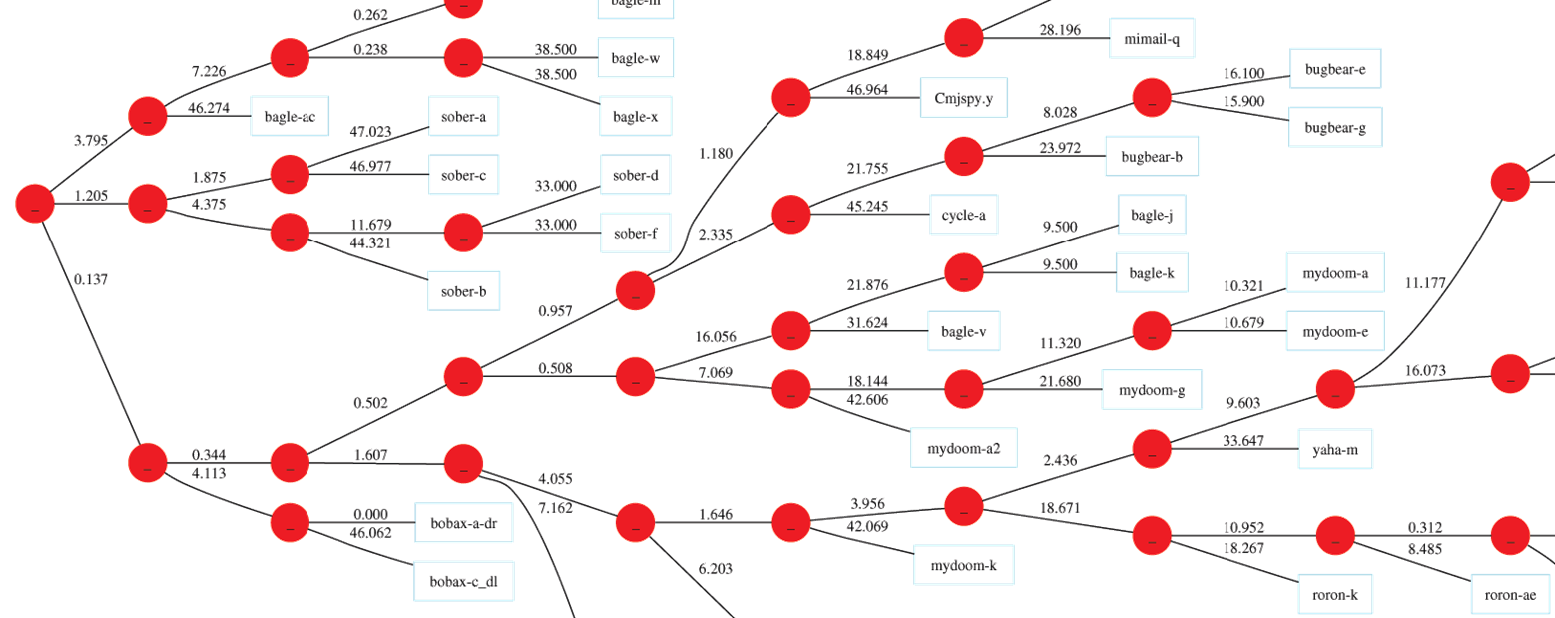
\includegraphics[scale=.50]{images/binary_diffing/xtree.png} \\
    \end{center}
\end{frame}


\subsection{Exercises}
\begin{frame}
    \frametitle{Exercise}
    \begin{itemize}
        \item Port work from Mydoom.D to Mydoom.M
        \item Any notable changes?
        \item Examine the differences between the dropped backdoors
    \end{itemize}
\end{frame}